\documentclass[paper=a4, fontsize=11pt]{scrreprt}

\usepackage[T1]{fontenc}
\usepackage[german]{babel}
\usepackage{amsfonts,amsthm, amsmath}
\usepackage{siunitx}
\usepackage[]{graphicx}
\usepackage{url}
\usepackage{floatrow}
\usepackage{sectsty}
\usepackage{fancyhdr}
\usepackage[utf8]{inputenc}

\allsectionsfont{\raggedright \normalfont\scshape}
\pagestyle{fancyplain}
\fancyhead{}
\fancyfoot[L]{}
\fancyfoot[C]{}
\fancyfoot[R]{\thepage}
\renewcommand{\headrulewidth}{0pt}
\renewcommand{\footrulewidth}{0pt}
\setlength{\headheight}{13.6pt}

\numberwithin{equation}{section}
\numberwithin{figure}{section} 
\numberwithin{table}{section}

\setlength\parindent{0pt}

\newcommand{\horrule}[1]{\rule{\linewidth}{#1}}

\title{	
	\normalfont \normalsize 
	\textsc{HAW, Praktikum Rechnernetze} \\ [25pt] 
	\horrule{0.5pt} \\[0.4cm]
	\huge Protokoll 01 \\
	\horrule{2pt} \\[0.5cm]
}

\author{Sebastian Wientzek, Daniel Schruhl}

\date{\normalsize\today}
\renewcommand{\thesection}{\arabic{section}}
\sisetup{range-phrase=--}
\begin{document}

\maketitle

\section{Webseitenabruf scimbe.de}

Der HTTP-Dialog (Schicht 7 OSI Referenzmodell, Anwendungsschicht) lässt sich grob in drei Phasen aufteilen: \textbf{Verbindungsaufbau}, \textbf{Datenaustausch}, \textbf{Verbindungsabbau}.

Das liegt daran, dass der HTTP-Dialog auf TCP (Schicht 4 OSI Referenzmodell, Transportschicht) basiert und verbindungsorientiert ist.\\

Der Verbindungsaufbau bei TCP erfolgt mittels des Drei-Wege-Handschlags (SYN, SYN /ACK, ACK).

Der Client sendet dem Server ein SYN-Paket, was der Server mit einem SYN/ACK-Paket bestätigt und somit dem Verbindungsaufbau zustimmt. Der Client bestätigt das wiederum mit einem ACK-Paket.\\

Am Anfang des Datenaustausches sendet der Client ein HTTP-Request an den Server. Dieser sendet nun die Antwort in mehreren Segmenten, welche einzeln vom Client bestätigt werden. 

Jedes Paket hat eine Sequenznummer, die nächste Sequenz Nummer und eine Länge, mit denen die Pakete wieder in Reihenfolge zusammengesetzt werden können (siehe Abbildung \ref{fig:tcp-package}) . Im letzten Segment wird ein HTTP-Response mit dem Code 200 vom Server an den Client gesendet, wo die einzelnen Segmente zusammengesetzt werden. Das wird ebenfalls vom Client mit einem ACK-Paket bestätigt.

Der Abbau (Teardown) wird durch ein FIN/ACK Paket signalisiert und von der Gegenstelle mit einem ACK Paket wiederum bestätigt. Das geschieht an beiden Endpunkten (Client und Server).

Beim Verbindungsabbau sendet der Client ein FIN/ACK-Paket an den Server, um die Verbindung Clientseitig zu beenden. Der Server bestätigt dies mit einem ACK-Paket und sendet ebenfalls ein FIN/ACK-Paket und beendet so die Verbindung Serverseitig, was zum Schluss vom Client mit einem ACK-Paket bestätigt wird.\\

Betrachtet man nun das http-Request Paket (Abbildung \ref{fig:http-package}) genauer, werden hier die verschiedenen Schichten klar:

\begin{center}
\begin{tabular}{|c|c|}
\hline 
 & \textbf{TCP/IP-Modell}\\ 
\hline 
Frame & Network Interface\\ 
\hline 
Ethernet II & Network Interface\\ 
\hline
Internet Protocol Version 4 & Internet\\ 
\hline
Transmission Control Protocol & Transport\\ 
\hline
Hypertext Transfer Protocol & Application\\ 
\hline 
\end{tabular}
\end{center}

Das Frame ist die physikalische Darstellung des gesamten Pakets. Im Ethernet werden die Quell- und Zieladresse als MAC-Adresse dargestellt. Da diese nicht direkt in einer IPv4 Adresse umgewandelt werden können, erfolgt eine Zuweisung über das Address Resolution Protocol (ARP). Über TCP wird die Kommunikation zwischen Quell- und Zieladresse festgelegt. Mittels HTTP werden letztendlich die Daten ausgetauscht.

\section{Webseitenabruf https://www.google.de}

Es ist generell kein großer Unterschied zum vorherigen Erscheinungsbild zu erkennen. Der einzige Unterschied besteht darin, dass das HTTP nicht mehr direkt eingebunden ist, sondern über das Secure Sockets Layer mit TLSv1.2 (siehe Abbildung \ref{fig:https-package}).\\

Nun beginnt der Nachrichtenaustausch allerdings in Form eines http-Request über ein "Handshake Protocol: Client Hello" und ein ACK-Paket, gefolgt von "Handshake Protocol: Server Hello" vom Server.

Als nächstes überträgt der Server uns in mehreren Segmenten ein Zertifikat, welches der Client mit einem ACK-Paket bestätigt. Der Client sendet darauf hin "Client Key Exchange, Change Cipher Spec".\\

Die weitere Kommunikation ist ab hier verschlüsselt. Sensible Daten, die nicht für die Kommunikation an sich benötigt werden, können so sicher ausgetauscht werden (siehe Abbildung \ref{fig:ssl-data}).

Die Verschlüsselung betrifft nur die überliegenden Schichten, also 5-7 im OSI Referenz Modell und die Application Layer im TCP/IP-Modell. Die darunterliegenden Schichten bleiben dabei lesbar.
\begin{center}
\begin{tabular}{|c|c|c|}
 \hline
 \textbf{Protokolle} & \textbf{TCP/IP-Modell} & \textbf{OSI-Referenzmodell} \\
 \hline
 Frame & Network Interface & Layer 1: Physical \\
 \hline
 Ethernet II & Network Interface & Layer 2: Data Link \\
 \hline
 Internet Protocol Version 4 & Internet & Layer 3: Network \\
 \hline
 Transmission Control Protocol & Transport & Layer 4: Transport\\
 \hline
 Secure Sockets Layer & Application &  Layer 7: Application\\
 \hline
\end{tabular}
\end{center}

\section{Webseitenabruf HTTP und HTTPS}

Beim Aufruf der HTTP-Adresse werden wir auf die Seite https://www.haw-hamburg.de/ti-i.html weitergeleitet.

Rufen wir direkt die HTTPS-Adresse auf, werden wir aufgefordert das Zertifikat zu akzeptieren und gelangen dann zu einem Raumbuchungssystem der HAW.

Da wir beim HTTP-Aufruf Port 80 anfragen, gibt uns der Server via HTTP den Code "302 Found" zurück mit einem Verweis auf die oben genannte Adresse, welche dann direkt aufgerufen wird.\\

Mit dem HTTPS-Aufruf wird allerdings direkt der Port 443 adressiert, wo es Serverseitig keine Weiterleitung auf die allgemeine Webseite gibt.

Der Dienstzugang (Port) für HTTPS und HTTPS ist also unterschiedlich (Port 80, 443) und im Server findet intern eine Weiterleitung statt, je nachdem aus welchem Netz man kommt und welchen Dienstzugang man anfragt. Diese Ports sind Well Known Ports. Das sind die Ports, die einen Zugang mit privilegierten Rechten benötigen (SUDO).

\section{IP-Adressen und Pings}

\subsection{IP-Adressen, Netzadressen, Broadcastadressen}

Mit dem Befehl \texttt{ifconfig} konnten wir neben dem Interface auch die IP-Adresse und Netzmaske abrufen. Die Netzadresse und Broadcastadresse haben wir manuell berechnet.

\begin{center}
\begin{tabular}{|c|c|c|c|c|}
\hline
\textbf{Interface} & IP-\textbf{Adresse} & \textbf{Netzmaske} & \textbf{Netzadresse} & \textbf{Broadcastadresse}\\
\hline
eth0 & 141.22.27.104 & 255.255.254.0 & 141.22.26.0 & 141.22.27.255 \\
\hline
eth1 & 192.168.18.131 & 255.255.255.0 & 192.168.18.0	 & 192.168.18.255 \\
\hline
eth2 & 172.16.1.7 & 255.255.255.0 & 172.16.1.0 & 172.16.1.255 \\
\hline
lo & 127.0.0.1 & 255.0.0.0 & 127.0.0.0 & 127.255.255.255 \\
\hline
\end{tabular}
\end{center}

\subsection{Pings}		

Beim ping unserer Loopback-Adresse (lo) haben wir selbst – wie erwartet - auch wieder geantwortet.\\

Bei einen ping auf die Broadcast-Adresse 141.22.27.255 (eth0) haben verschiedene Teilnehmer des Subnetzes geantwortet, wobei häufig ein "(DUP!)" für Duplikate als Hinweis mit ausgegeben wurde.\\

Zuerst gab es bei einen ping auf die Broadcast-Adresse 192.168.18.255 (eth1) keine Antwort, da die entsprechenden Netzwerkkomponenten (Switch) nicht eingeschaltet waren. 

Nachdem das von der Praktikumsleitung behoben wurde, gab es entgegen unserer Erwartung nur zwei Teilnehmer die antworteten.

Einsicht bat uns der Netzwerk Plan von Herrn Hartmut Schulz. Wir stellten fest, dass nur ein ISDN-Router und ein Switch antworteten. Außerdem waren alle anderen lokalen Teilnehmer im selben Netz ausgeschaltet.\\

Ein ping auf die Broadcast-Adresse 172.16.1.255 (eth2) ergab erneut keinerlei Antworten anderer Teilnehmer, obwohl wir mithilfe eines Mitstudierenden, der Praktikumsleitung und Wireshark bestätigen konnten, dass die ping Anfragen bei anderen Teilnehmern ankamen. Im weiteren Verlauf des Praktikums konnte leider nicht geklärt werden, weshalb es keine Antwort auf den ping gab.

\newpage

\section{Anhang}

\begin{figure}[!htb] 
  \centering
     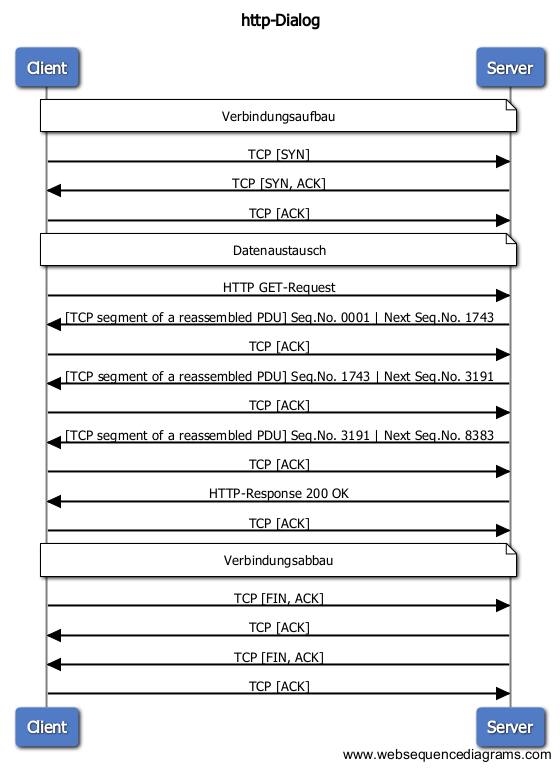
\includegraphics[width=0.5\textwidth]{resources/http-Dialog.png}
  \caption{Message Sequence Chart http-Dialog}
  \label{fig:http-dialog}
\end{figure}

\begin{figure}[!htb] 
  \centering
     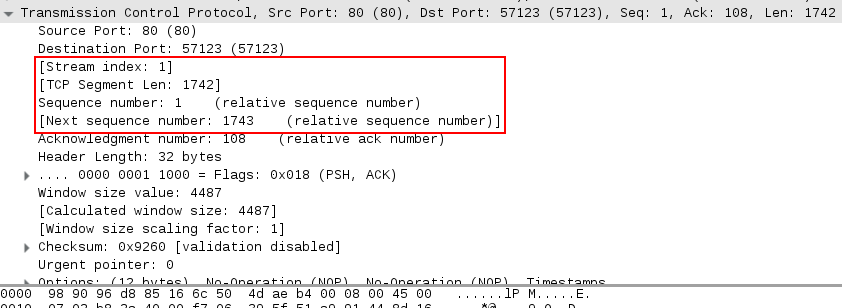
\includegraphics[width=1.0\textwidth]{resources/tcp-package.png}
  \caption{TCP Paket}
  \label{fig:tcp-package}
\end{figure}

\begin{figure}[!htb] 
  \centering
     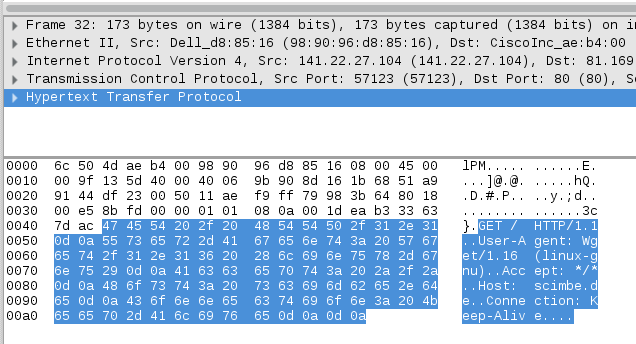
\includegraphics[width=0.7\textwidth]{resources/paket-http.png}
  \caption{HTTP-Request Paket}
  \label{fig:http-package}
\end{figure}

\begin{figure}[!htb] 
  \centering
     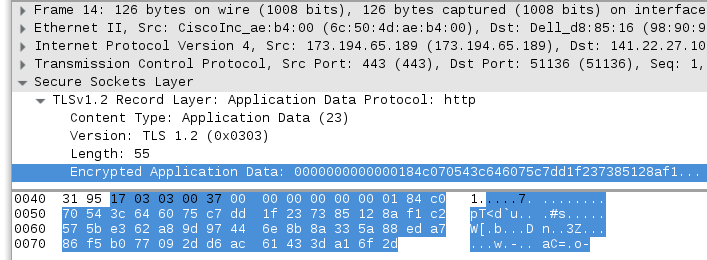
\includegraphics[width=0.7\textwidth]{resources/https-package.png}
  \caption{HTTP-Request Paket mit SSL}
  \label{fig:https-package}
\end{figure}

\begin{figure}[!htb] 
  \centering
     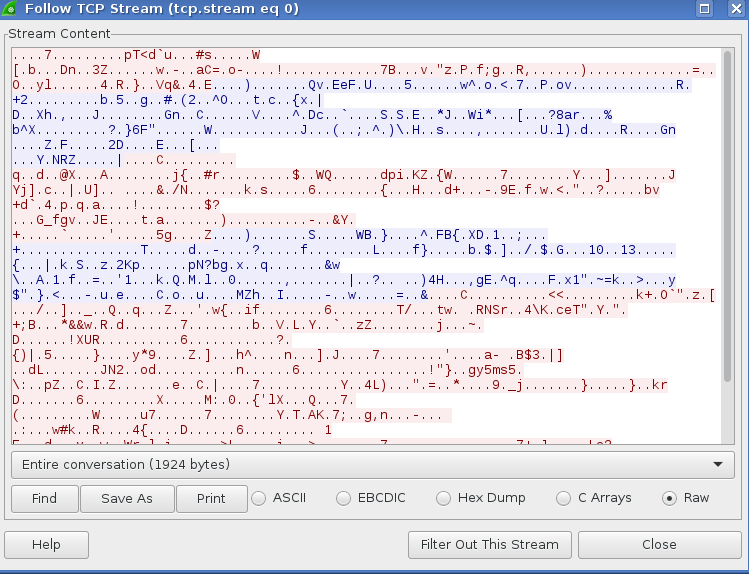
\includegraphics[width=0.7\textwidth]{resources/ssl-data.png}
  \caption{Verschlüsselter Inhalt}
  \label{fig:ssl-data}
\end{figure}

\begin{figure}[!htb] 
  \centering
     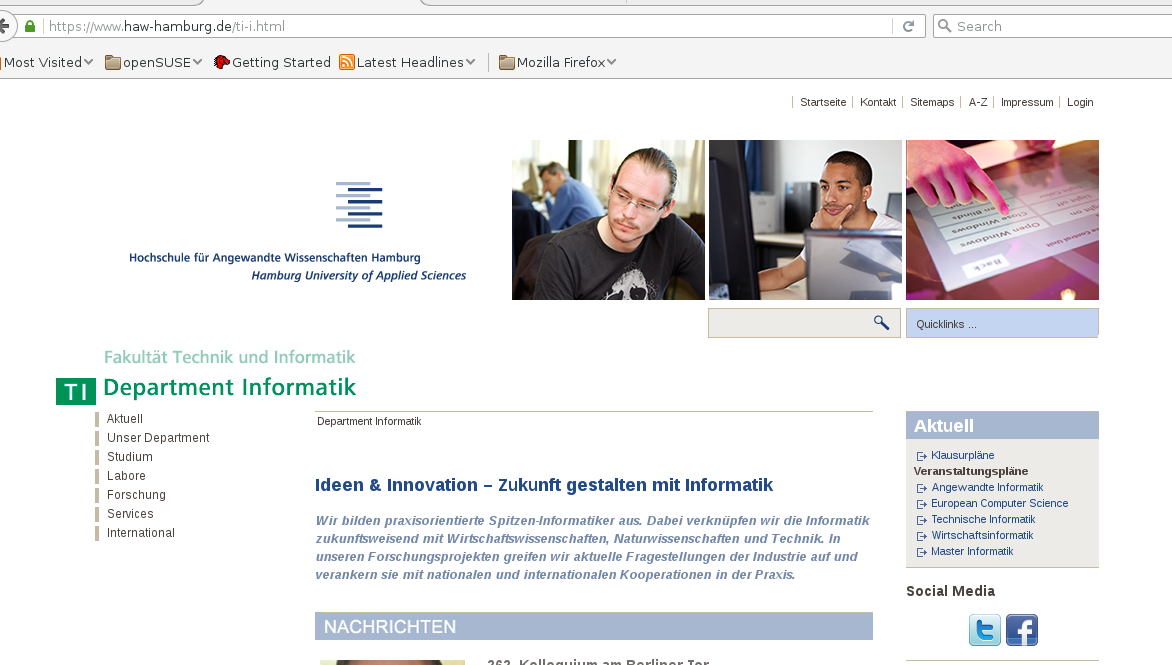
\includegraphics[width=1.0\textwidth]{resources/http-aufruf.png}
  \caption{Aufruf der Seite http://www.informatik.haw-hamburg.de/}
  \label{fig:http-site}
\end{figure}

\begin{figure}[!htb] 
  \centering
     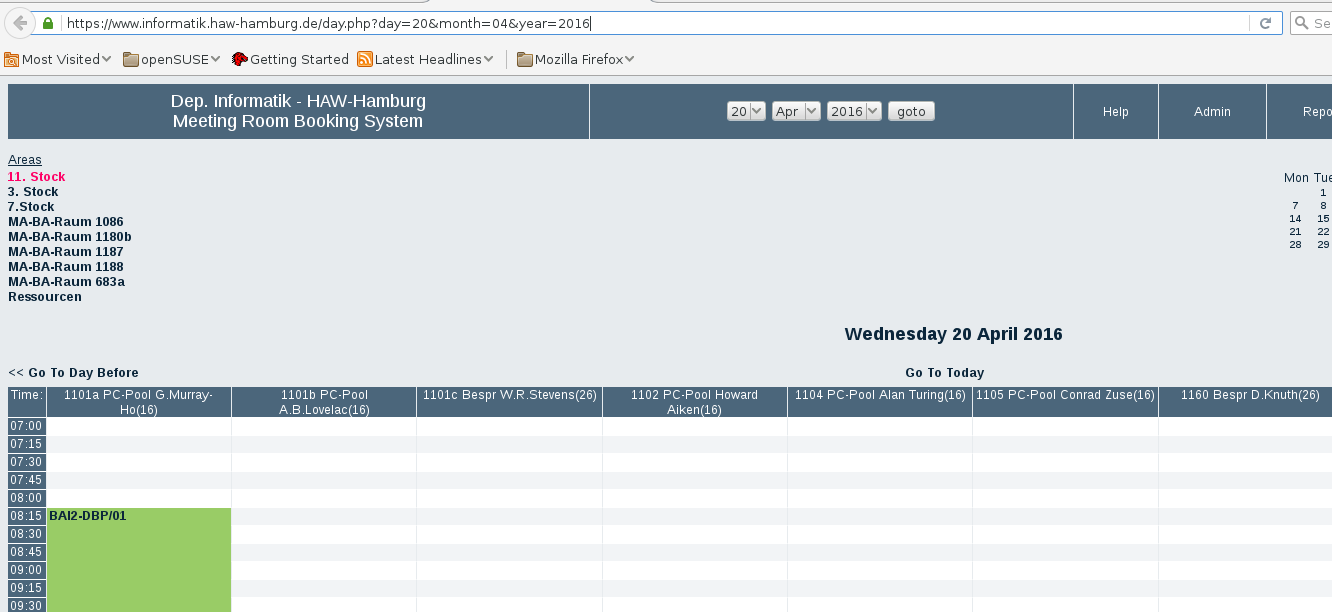
\includegraphics[width=1.0\textwidth]{resources/https-aufruf.png}
  \caption{Aufruf der Seite https://www.informatik.haw-hamburg.de/}
  \label{fig:https-site}
\end{figure}

\end{document}